%
% Portuguese-BR vertion
% 
\documentclass{article}

\usepackage{ipprocess}
% Use longtable if you want big tables to split over multiple pages.
% \usepackage{longtable}
\usepackage[utf8]{inputenc} 
\usepackage[brazil]{babel} % Uncomment for portuguese

\sloppy

\graphicspath{{./pictures/}} % Pictures dir
\makeindex
\begin{document}

\DocumentTitle{Documento de Casos de Uso}
\Project{Core-MUSA}
\Organization{Universidade Estadual de Feira de Santana}
\Version{Build 1}

\capa
\newpage

%%%%%%%%%%%%%%%%%%%%%%%%%%%%%%%%%%%%%%%%%%%%%%%%%%
%% Revision History
%%%%%%%%%%%%%%%%%%%%%%%%%%%%%%%%%%%%%%%%%%%%%%%%%%
\section*{\center Histórico de Revisões}
  \vspace*{1cm}
  \begin{table}[ht]
    \centering
    \begin{tabular}[pos]{|m{2cm} | m{7.2cm} | m{3.8cm}|} 
      \hline
      \cellcolor[gray]{0.9}
      \textbf{Date} & \cellcolor[gray]{0.9}\textbf{Descrição} & \cellcolor[gray]{0.9}\textbf{Autor(s)}\\ \hline
      \hline
      \small 08/10/2014 & \small Concepção do documento & \small 
      \begin{itemize}
      	\item bezourokq;
      	\item wsbittencourt;
      	\item fmbboaventura;  
	  \end{itemize}      	
      \\ \hline 
    \end{tabular}
  \end{table}

\newpage

% TOC instantiation
\tableofcontents
\newpage

%%%%%%%%%%%%%%%%%%%%%%%%%%%%%%%%%%%%%%%%%%%%%%%%%%
%% Document main content
%%%%%%%%%%%%%%%%%%%%%%%%%%%%%%%%%%%%%%%%%%%%%%%%%%
\section{Introdução}

  \subsection{Objetivo}
  
  \subsection{Visão Geral do Documento}
  \begin{itemize}
    \item Sessão 2: lista todos os possíveis atores do sistema.
    \item Sessão 3: relata a lista dos casos de uso do projeto.
    % \item Referências: provê uma lista completa de todos os artefatos referenciados nesse documento.
  \end{itemize}
  
  \subsection{Representação Simbólica}
  A Figura \ref{fig:uc_exemple} ilustra a simbologia utilizada para representar operações que devem ser realizadas pelo sistema. A Figura \ref{fig:actors} ilustra as duas simbologias utilizadas para representar os Atores do sistema. Um ator, dentro do escopo desta descrição, pode ser identificado como um módulo \textit{top level}, ou como um elemento de entrada e saída (botões, sensores, displays, etc).
  
  \FloatBarrier
  \begin{figure}[H]
    \centering
    
\includegraphics[width=0.25\textwidth]{uc_exemple.png}
    \caption{Exemplo de Caso de Uso.}
    \label{uc_exemple}
  \end{figure}  
  
  A simbologia usual para representação de um Ator é apresentada na Figura \ref{fig:actor_exemple}, no entanto, para representar módulos incorporados que outrora deveriam utilizar a mesma simbologia, utiliza-se a representação ilustrada nas Figuras \ref{fig:ipcore_exemple} e \ref{fig:ipcore_single_exemple}, definida por convenção. Este elemento, em geral, está associado aos módulos do sistema, ou IP-cores de terceiros incorporados ao mesmo. Esta simbologia ainda foi divida, tendo em vista representar instâncias únicas (Figura \ref{fig:ipcore_single_exemple}), ou múltiplas (Figura \ref{fig:ipcore_exemple}) de um determinado componente. 
  
  \FloatBarrier
  \begin{figure}[H]
    \centering
    \begin{subfigure}[b]{0.3\textwidth}
      \centering
      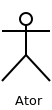
\includegraphics[width=0.25\textwidth]{actor_exemple.png}
      \caption{Ator do Sistema.}
      \label{fig:actor_exemple}
    \end{subfigure} 
    \begin{subfigure}[b]{0.3\textwidth}
      \centering
      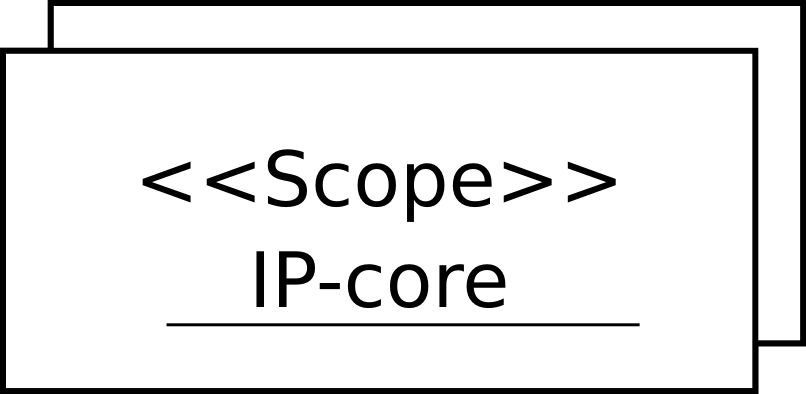
\includegraphics[width=0.6\textwidth]{ipcore_exemple.png}
      \caption{Instância múltipla de um IP.}
      \label{fig:ipcore_exemple}
    \end{subfigure}
    \begin{subfigure}[b]{0.3\textwidth}
      \centering
      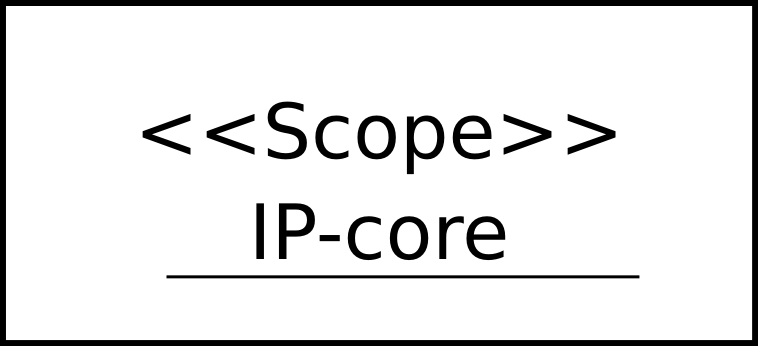
\includegraphics[width=0.6\textwidth]{ipcore_single_exemple.png}
      \caption{Instância de um IP.}
      \label{fig:ipcore_single_exemple}
    \end{subfigure}
    \caption{Simbologia utilizada na implementação dos Casos de Uso.}
    \label{fig:actors}
  \end{figure}
  
  O projetista responsável por interpretar os diagramas não deve confundir-se no momento de interpretar as simbologias de atores. A representação alternativa, não implica que o módulo será instanciado no subsistema em questão, mas sim que os recursos providos por este \textit{core} são necessários para garantir o seu funcionamento.
  
  \subsection{Definições, Acrônimos e Abreviações}
  \FloatBarrier
    \begin{table}[H] 
      \begin{center}
        \begin{tabular}[pos]{|m{2cm} | m{8cm}|} 
          \hline 
          \cellcolor[gray]{0.9}\textbf{Termo} & \cellcolor[gray]{0.9}\textbf{Descrição} \\ \hline
          UC & Caso de Uso  \\ \hline
          SB & Sub-fluxo \\ \hline
          FS & Fluxo Secundário \\ \hline
          NFR & Requisito Não Funcional \\ \hline
          FR & Requisito Funcional \\ \hline
          BT & Botão Direcional \\
          \hline
        \end{tabular}
      \end{center}
    \label{tab:definicoes}
    \end{table}

  \section{Atores do Sistema}
  
\begin{figure}[htb]
\centering
\begin{minipage}[c]{0.19\linewidth}
\centering
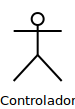
\includegraphics[scale=0.50]{./pictures/use/atores/controlador.png}
\end{minipage}
\begin{minipage}[c]{0.19\linewidth}
\centering
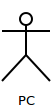
\includegraphics[scale=0.50]{./pictures/use/atores/pc.png}
\end{minipage}
\begin{minipage}[c]{0.19\linewidth}
\centering
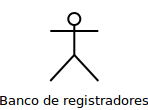
\includegraphics[scale=0.50]{./pictures/use/atores/banco_registradores.png}
\end{minipage}
\begin{minipage}[c]{0.19\linewidth}
\centering
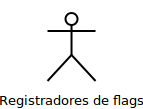
\includegraphics[scale=0.50]{./pictures/use/atores/reistradores_flags.png}
\end{minipage}
\end{figure}

\textbf{Controlador} – Unidade que controla a execução das operações.

\textbf{PC} – Registrador contador e programa, aponta para próxima instrução.

\textbf{Banco de registradores} – Conjunto de registradores de uso geral.

\textbf{Registradores de flags} – Registradores de uso específicos para sinalizar resultados de operações.
  
  \section{Casos de Usos}
  Esta sessão apresenta o conjunto de UC realizados para a implementação do projeto \textit{Core MUSA} (Núcleo de processamento de instruções do processador de propósito geral MUSA). As sessões a seguir foram divididas e nomeada utilizando a nomenclatura abreviada [UC (NÚMERO DO UC)] seguido de uma breve descrição em forma de título.

  \usecase{Decodifica instrução}
  O controlador é responsável por decodificar instrução e emitir resultado de operações aos registradores.
  
  \actors
    \begin{description}
     \item \textbf{PC} – Registrador contador e programa, aponta para próxima instrução.
     \item \textbf{Banco de registradores} – Conjunto de registradores de uso geral.
    \end{description}
    
  \preconditions 
    \begin{itemize}
     \item Atender aos requisitos funcionais [FR01 e FR02];
     \item Leitura do PC;
    \end{itemize}

  \postconditions
    \begin{itemize}
     \item Os resultados devem ser expressos nos registradores.
    \end{itemize}
  
  \ucdiagram{./pictures/use/case/leitura.png}
  
  % descricao do fluxo principal de eventos
  \begin{mainflow}
    \item Acesso ao PC;
    \item Acesso aos respectivos registradores;
    \item Executa operações;
    \item Atualiza registradores;
  \end{mainflow}
  
  % descricao do fluxo secundário (quando existir)
  %\begin{secondaryflow} 
   % \sfitem{Título do Fluxo Secundário}
    %\begin{enumerate}
     % \item Liste aqui as etapas do fluxo secundário;
    %\end{enumerate}
    %\sfitem{Título do Fluxo Secundário}
    %\begin{enumerate}
     % \item Liste aqui as etapas do fluxo secundário;
    %\end{enumerate}
  %\end{secondaryflow}  

% Optional bibliography section
% To use bibliograpy, first provide the ipprocess.bib file on the root folder.
% \bibliographystyle{ieeetr}
% \bibliography{ipprocess}

\end{document}
